% answers.tex —— 2008 年·全国大纲卷Ⅰ·理科 · 参考答案与详细解析片段
% 由 tools/generate_projects.py 依来源总账自 2008/2008_数学真题_全国1理_试题.md + 2008/2008_数学真题_全国1理_解析正文.md + 2008/2008_数学真题_全国1理_答案要点.md 生成，勿手改（改源 MD 后重跑）


\begin{gktip}
固定源 PDF 为印刷页码 433–434 的两页题面，不附答案。以下解析均依据固定源独立复算；第 2、12、18 题图形在 LaTeX 工程中以 TikZ/PGFPlots 矢量源重绘。
\end{gktip}

\begin{answer}
\gksolhead{1}{}

\textbf{题目}：

函数 $y=\sqrt{x(x-1)}+\sqrt{x}$ 的定义域为\mbox{（　　）}

（A）$\{x\mid x\geqslant0\}$\quad（B）$\{x\mid x\geqslant1\}$\quad（C）$\{x\mid x\geqslant1\}\cup\{0\}$\quad（D）$\{x\mid0\leqslant x\leqslant1\}$

\Needspace{4\baselineskip}
\textbf{解析}

要求 $x\geqslant0$ 且 $x(x-1)\geqslant0$，故 $x=0$ 或 $x\geqslant1$，选 C。

\gkanswer{答案：C}

\end{answer}
\begin{answer}
\gksolhead{2}{}

\textbf{题目}：

汽车经过启动、加速行驶、匀速行驶、减速行驶之后停车，若把这一过程中汽车的行驶路程 $s$ 看作时间 $t$ 的函数，其图象可能是\mbox{（　　）}
\nopagebreak[4]
\begin{center}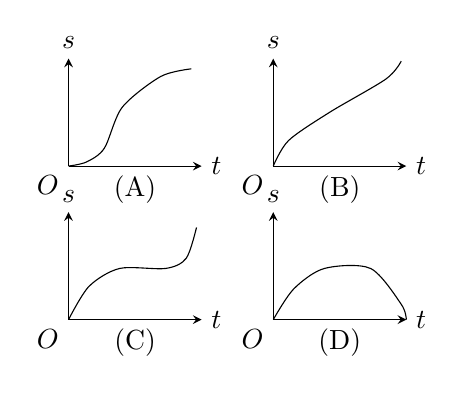
\begin{tikzpicture}[>=stealth,scale=.65]
\foreach \x/\y/\lab in {0/0/A,4/0/B,0/-3/C,4/-3/D}{
  \begin{scope}[shift={(\x,\y)}]
    \draw[->] (0,0)--(2.6,0) node[right] {$t$};
    \draw[->] (0,0)--(0,2.1) node[above] {$s$};
    \node[below left] at (0,0) {$O$};
    \node at (1.3,-.45) {(\lab)};
  \end{scope}
}
\draw plot[smooth] coordinates {(0,0) (.35,.08) (.7,.35) (1.05,1.15) (1.8,1.75) (2.4,1.9)};
\draw[shift={(4,0)}] plot[smooth] coordinates {(0,0) (.3,.5) (1.1,1.05) (2.2,1.7) (2.5,2.05)};
\draw[shift={(0,-3)}] plot[smooth] coordinates {(0,0) (.4,.65) (1.0,1.0) (1.9,1.0) (2.3,1.2) (2.5,1.8)};
\draw[shift={(4,-3)}] plot[smooth] coordinates {(0,0) (.4,.6) (1.0,1.0) (1.9,1.0) (2.5,.3) (2.6,0)};
\end{tikzpicture}
\end{center}
\nopagebreak[4]
（A）图 A\quad（B）图 B\quad（C）图 C\quad（D）图 D

\Needspace{4\baselineskip}
\textbf{解析}

路程函数的斜率是速度，启动、加速、匀速、减速对应斜率先增大、保持、减小到零，图象选 A。

\gkanswer{答案：A}

\end{answer}
\begin{answer}
\gksolhead{3}{}

\textbf{题目}：

在 $\triangle ABC$ 中，$\overrightarrow{AB}=\boldsymbol c$，$\overrightarrow{AC}=\boldsymbol b$。若点 $D$ 满足 $\overrightarrow{BD}=2\overrightarrow{DC}$，则 $\overrightarrow{AD}=$\mbox{（　　）}

（A）$\dfrac23\boldsymbol b+\dfrac13\boldsymbol c$\quad（B）$\dfrac53\boldsymbol c-\dfrac23\boldsymbol b$\quad（C）$\dfrac23\boldsymbol b-\dfrac13\boldsymbol c$\quad（D）$\dfrac13\boldsymbol b+\dfrac23\boldsymbol c$

\Needspace{4\baselineskip}
\textbf{解析}

\Needspace{5\baselineskip}
由 $\overrightarrow{BD}=2\overrightarrow{DC}$，得

\nopagebreak[4]
\[
\overrightarrow{AD}
=\overrightarrow{AB}+\overrightarrow{BD}
=\frac23\boldsymbol b+\frac13\boldsymbol c
\]

选项中对应 C。

\gkanswer{答案：A}

\end{answer}
\begin{answer}
\gksolhead{4}{}

\textbf{题目}：

设 $a\in\mathbb R$，且 $(a+\mathrm i)^2\mathrm i$ 为正实数，则 $a=$\mbox{（　　）}

（A）$2$\quad（B）$1$\quad（C）$0$\quad（D）$-1$

\Needspace{4\baselineskip}
\textbf{解析}

\nopagebreak[4]
\[
(a+\mathrm i)^2\mathrm i=-2a+(a^2-1)\mathrm i
\]

为正实数要求 $a^2-1=0$ 且 $-2a>0$，故 $a=-1$，选 D。

\gkanswer{答案：D}

\end{answer}
\begin{answer}
\gksolhead{5}{}

\textbf{题目}：

已知等差数列 $\{a_n\}$ 满足 $a_2+a_4=4$，$a_3+a_5=10$，则它的前 $10$ 项的和 $S_{10}=$\mbox{（　　）}

（A）$138$\quad（B）$135$\quad（C）$95$\quad（D）$23$

\Needspace{4\baselineskip}
\textbf{解析}

\Needspace{5\baselineskip}
设首项为 $a_1$、公差为 $d$，则

\nopagebreak[4]
\[
a_1+2d=2,\qquad a_1+3d=5
\]

\Needspace{5\baselineskip}
得 $d=3,a_1=-4$，从而

\nopagebreak[4]
\[
S_{10}=5(2a_1+9d)=95
\]

选 C。

\gkanswer{答案：C}

\end{answer}
\begin{answer}
\gksolhead{6}{}

\textbf{题目}：

若函数 $y=f(x-1)$ 的图象与函数 $y=\ln\sqrt{x}+1$ 的图象关于直线 $y=x$ 对称，则 $f(x)=$\mbox{（　　）}

（A）$e^{2x-1}$\quad（B）$e^{2x}$\quad（C）$e^{2x+1}$\quad（D）$e^{2x+2}$

\Needspace{4\baselineskip}
\textbf{解析}

先求 $y=\ln\sqrt{x}+1$ 的反函数，得 $g(x)=e^{2x-2}$。题设 $f(x-1)=g(x)$，所以 $f(x)=g(x+1)=e^{2x}$，选 B。

\gkanswer{答案：B}

\end{answer}
\begin{answer}
\gksolhead{7}{}

\textbf{题目}：

设曲线 $y=\dfrac{x+1}{x-1}$ 在点 $(3,2)$ 处的切线与直线 $ax+y+1=0$ 垂直，则 $a=$\mbox{（　　）}

（A）$2$\quad（B）$\dfrac12$\quad（C）$-\dfrac12$\quad（D）$-2$

\Needspace{4\baselineskip}
\textbf{解析}

\Needspace{5\baselineskip}
曲线斜率为

\nopagebreak[4]
\[
y'=-\frac2{(x-1)^2}
\]

在 $x=3$ 处为 $-1/2$。直线 $ax+y+1=0$ 斜率为 $-a$，两直线垂直得 $a=2$，选 A。

\gkanswer{答案：A}

\end{answer}
\begin{answer}
\gksolhead{8}{}

\textbf{题目}：

为得到函数 $y=\cos\left(2x+\dfrac\pi3\right)$ 的图象，只需将函数 $y=\sin2x$ 的图象\mbox{（　　）}

（A）向左平移 $\dfrac{5\pi}{12}$ 个长度单位\quad（B）向右平移 $\dfrac{5\pi}{12}$ 个长度单位\quad（C）向左平移 $\dfrac{5\pi}{6}$ 个长度单位\quad（D）向右平移 $\dfrac{5\pi}{6}$ 个长度单位

\Needspace{4\baselineskip}
\textbf{解析}

\nopagebreak[4]
\[
\cos\left(2x+\frac\pi3\right)=\sin\left(2x+\frac{5\pi}6\right)
\]

故应向左平移 $5\pi/12$，选 A。

\gkanswer{答案：A}

\end{answer}
\begin{answer}
\gksolhead{9}{}

\textbf{题目}：

设奇函数 $f(x)$ 在 $(0,+\infty)$ 上为增函数，且 $f(1)=0$，则不等式 $\dfrac{f(x)-f(-x)}{x}<0$ 的解集为\mbox{（　　）}

（A）$(-1,0)\cup(1,+\infty)$\quad（B）$(-\infty,-1)\cup(0,1)$\quad（C）$(-\infty,-1)\cup(1,+\infty)$\quad（D）$(-1,0)\cup(0,1)$

\Needspace{4\baselineskip}
\textbf{解析}

奇函数给出 $f(-x)=-f(x)$。当 $x>0$ 时，不等式等价于 $f(x)<0$，即 $0<x<1$；当 $x<0$ 时得到 $-1<x<0$，故选 D。

\gkanswer{答案：D}

\end{answer}
\begin{answer}
\gksolhead{10}{}

\textbf{题目}：

若直线 $\dfrac{x}{a}+\dfrac{y}{b}=1$ 通过点 $M(\cos\alpha,\sin\alpha)$，则\mbox{（　　）}

（A）$a^2+b^2\leqslant1$\quad（B）$a^2+b^2\geqslant1$\quad（C）$\dfrac1{a^2}+\dfrac1{b^2}\leqslant1$\quad（D）$\dfrac1{a^2}+\dfrac1{b^2}\geqslant1$

\Needspace{4\baselineskip}
\textbf{解析}

\Needspace{5\baselineskip}
单位圆上存在点满足 $\cos\alpha/a+\sin\alpha/b=1$，当且仅当

\nopagebreak[4]
\[
\sqrt{\frac1{a^2}+\frac1{b^2}}\geqslant1
\]

即 $\dfrac1{a^2}+\dfrac1{b^2}\geqslant1$，选 D。

\gkanswer{答案：D}

\end{answer}
\begin{answer}
\gksolhead{11}{}

\textbf{题目}：

已知三棱柱 $ABC-A_1B_1C_1$ 的侧棱与底面边长都相等，$A_1$ 在底面 $ABC$ 内的射影为 $\triangle ABC$ 的中心，则 $AB_1$ 与底面 $ABC$ 所成角的正弦值等于\mbox{（　　）}

（A）$\dfrac13$\quad（B）$\dfrac{\sqrt2}{3}$\quad（C）$\dfrac{\sqrt3}{3}$\quad（D）$\dfrac23$

\Needspace{4\baselineskip}
\textbf{解析}

与全国Ⅰ文科第 11 题同样坐标化，侧棱竖直分量为 $\sqrt{2/3}$，$AB_1$ 长为 $\sqrt3$，故线面角正弦为 $\sqrt2/3$，选 B。

\gkanswer{答案：B}

\end{answer}
\begin{answer}
\gksolhead{12}{}

\textbf{题目}：

如图，一环形花坛分成 $A\text{、}B\text{、}C\text{、}D$ 四块，现有 $4$ 种不同的花供选种，要求在每块里种 $1$ 种花，且相邻的 $2$ 块种不同的花，则不同的种法总数为\mbox{（　　）}
\nopagebreak[4]
\begin{center}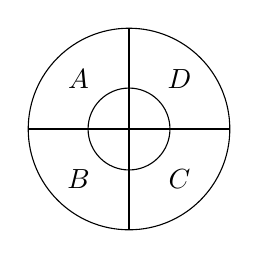
\begin{tikzpicture}[scale=.8]
\draw (0,0) circle (1.6);
\draw (0,0) circle (.65);
\draw (-1.6,0)--(1.6,0) (0,-1.6)--(0,1.6);
\node at (-.8,.8) {$A$}; \node at (.8,.8) {$D$};
\node at (-.8,-.8) {$B$}; \node at (.8,-.8) {$C$};
\end{tikzpicture}
\end{center}
\nopagebreak[4]
（A）$96$\quad（B）$84$\quad（C）$60$\quad（D）$48$

\Needspace{4\baselineskip}
\textbf{解析}

\Needspace{5\baselineskip}
环形四块相邻关系构成四边形。先选 A 有 $4$ 种，选 B 有 $3$ 种；若 C 与 A 同色，D 有 $3$ 种，否则 D 有 $2$ 种，合计

\nopagebreak[4]
\[
4\cdot3\cdot(1\cdot3+2\cdot2)=84
\]

选 B。

\gkanswer{答案：B}

\end{answer}
\begin{answer}
\gksolhead{13}{}

\textbf{题目}：

\Needspace{5\baselineskip}
若 $x,y$ 满足约束条件

\nopagebreak[4]
\[
\begin{cases}
x+y\geqslant0,\\
x-y+3\geqslant0,\\
0\leqslant x\leqslant3,
\end{cases}
\]

则 $z=2x-y$ 的最大值为\gkblank{}。

\Needspace{4\baselineskip}
\textbf{解析}

可行域与文科第 13 题相同，顶点 $(0,0),(0,3),(3,-3),(3,6)$ 中在 $(3,-3)$ 处 $z=9$ 最大。

\gkanswer{答案：$9$}

\end{answer}
\begin{answer}
\gksolhead{14}{}

\textbf{题目}：

已知抛物线 $y=ax^2-1$ 的焦点是坐标原点，则以抛物线与两坐标轴的三个交点为顶点的三角形面积为\gkblank{}。

\Needspace{4\baselineskip}
\textbf{解析}

抛物线焦点为原点给出 $a=1/4$，与坐标轴交点为 $(\pm2,0),(0,-1)$，三角形面积为 $2$。

\gkanswer{答案：$2$}

\end{answer}
\begin{answer}
\gksolhead{15}{}

\textbf{题目}：

在 $\triangle ABC$ 中，$AB=BC$，$\cos B=-\dfrac7{18}$。若以 $A\text{、}B$ 为焦点的椭圆经过点 $C$，则该椭圆的离心率 $e=$\gkblank{}。

\Needspace{4\baselineskip}
\textbf{解析}

\Needspace{5\baselineskip}
设 $AB=BC=s$。由余弦定理

\nopagebreak[4]
\[
AC=s\sqrt{2-2\cos B}=s\sqrt{\frac{50}{18}}=\frac53s
\]

椭圆焦点为 $A,B$ 且过 $C$，所以 $2a=AC+BC=8s/3$，$2c=AB=s$，故 $e=3/8$。

\gkanswer{答案：$\dfrac38$}

\end{answer}
\begin{answer}
\gksolhead{16}{}

\textbf{题目}：

等边三角形 $ABC$ 与正方形 $ABDE$ 有一公共边 $AB$，二面角 $C-AB-D$ 的余弦值为 $\dfrac{\sqrt3}{3}$，$M\text{、}N$ 分别是 $AC\text{、}BC$ 的中点，则 $EM\text{、}AN$ 所成角的余弦值等于\gkblank{}。

\Needspace{4\baselineskip}
\textbf{解析}

\Needspace{5\baselineskip}
取 $AB=1$，设正方形所在平面内从 $A$ 出发的单位向量为 $\boldsymbol u$，其与等边三角形所在平面的二面角余弦为 $\sqrt3/3$。用坐标计算中点向量 $\overrightarrow{EM}$、$\overrightarrow{AN}$，得

\nopagebreak[4]
\[
|\overrightarrow{EM}|=|\overrightarrow{AN}|=\frac{\sqrt3}{2},\qquad
\overrightarrow{EM}\cdot\overrightarrow{AN}=\frac18
\]

故所成角余弦为 $1/6$。

\gkanswer{答案：$\dfrac16$}

\end{answer}
\begin{answer}
\gksolhead{17}{}

\textbf{题目}：

设 $\triangle ABC$ 的内角 $A\text{、}B\text{、}C$ 所对的边长分别为 $a\text{、}b\text{、}c$，且 $a\cos B-b\cos A=\dfrac35c$，$b\sin A=4$。

（1） 求 $\tan A\cot B$ 的值；

（2） 求 $\tan(A-B)$ 的最大值。

\Needspace{4\baselineskip}
\textbf{解析}

\gksubpart{(1)}

\Needspace{5\baselineskip}
由正弦定理，$a\sin B=b\sin A$，结合 $b\sin A=4$ 得 $a\sin B=4$。题设 $a\cos B-b\cos A=3c/5$，用 $a=2R\sin A,b=2R\sin B,c=2R\sin C$ 化为

\nopagebreak[4]
\[
\frac{\sin A\cos B-\sin B\cos A}{\sin(A+B)}
=\frac35
\]

\Needspace{5\baselineskip}
即

\nopagebreak[4]
\[
\frac{\tan A-\tan B}{\tan A+\tan B}=\frac35
\]

所以 $\tan A=4\tan B$，从而 $\tan A\cot B=4$。令 $t=\tan B$，则

\gksubpart{(2)}

\nopagebreak[4]
\[
\tan(A-B)=\frac{3t}{1+4t^2}\leqslant\frac34
\]

最大值为 $3/4$。

\gkanswer{答案（1）：$\tan A\cot B=4$。}

\gkanswer{答案（2）：$\tan(A-B)$ 的最大值为 $\dfrac34$。}

\end{answer}
\begin{answer}
\gksolhead{18}{}

\textbf{题目}：

四棱锥 $A-BCDE$ 中，底面 $BCDE$ 为矩形，侧面 $ABC\perp$ 底面 $BCDE$，$BC=2$，$CD=\sqrt2$，$AB=AC$。
\nopagebreak[4]
\begin{center}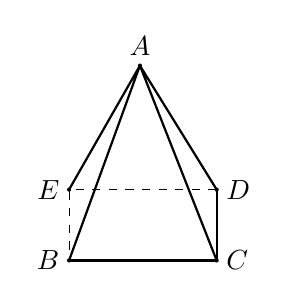
\begin{tikzpicture}[scale=.75,>=stealth]
\coordinate (B) at (0,0); \coordinate (C) at (2.5,0);
\coordinate (D) at (2.5,1.2); \coordinate (E) at (0,1.2);
\coordinate (A) at (1.2,3.3);
\draw[thick] (B)--(C)--(D); \draw[dashed] (D)--(E)--(B);
\draw[thick] (A)--(B) (A)--(C) (A)--(D) (A)--(E);
\draw[dashed] (A)--(D);
\fill (A) circle (1pt) node[above] {$A$};
\fill (B) circle (1pt) node[left] {$B$};
\fill (C) circle (1pt) node[right] {$C$};
\fill (D) circle (1pt) node[right] {$D$};
\fill (E) circle (1pt) node[left] {$E$};
\end{tikzpicture}
\end{center}
\nopagebreak[4]
（1） 证明：$AD\perp CE$；

（2） 设 $CE$ 与平面 $ABE$ 所成的角为 $45^\circ$，求二面角 $C-AD-E$ 的大小。

\Needspace{4\baselineskip}
\textbf{解析}

\gksubpart{(1)}

\Needspace{5\baselineskip}
先按全国Ⅰ文科第 18 题坐标化，$AD\perp CE$。令 $A=(1,0,h)$，则

\nopagebreak[4]
\[
\sin\angle(CE,\text{\text{平面} }ABE)
=\frac{\sqrt{2/3}\,h}{\sqrt{h^2+1}}
\]

题设角为 $45^\circ$，解得 $h=\sqrt3$。代入两平面的法向量计算，二面角仍满足

\gksubpart{(2)}

\nopagebreak[4]
\[
\cos\theta=\frac1{\sqrt{10}}
\]

\gkanswer{答案（1）：$p=0.001$。}

\gkanswer{答案（2）：每位投保人的最低保费为 $15$ 元。}

\end{answer}
\begin{answer}
\gksolhead{19}{}

\textbf{题目}：

已知函数 $f(x)=x^3+ax^2+x+1$，$a\in\mathbb R$。

（1） 讨论函数 $f(x)$ 的单调区间；

（2） 设函数 $f(x)$ 在区间 $\left(-\dfrac23,-\dfrac13\right)$ 内是减函数，求 $a$ 的取值范围。

\Needspace{4\baselineskip}
\textbf{解析}

\gksubpart{(1)}

\Needspace{5\baselineskip}
函数导数

\nopagebreak[4]
\[
f'(x)=3x^2+2ax+1
\]

故当 $|a|\leqslant\sqrt3$ 时在全体实数上递增；当 $|a|>\sqrt3$ 时，以导数的两个根为界，函数依次递增、递减、递增。

\gksubpart{(2)}

对区间 $(-2/3,-1/3)$ 递减需两端导数均不正，得到 $a\geqslant2$。

\gkanswer{答案（1）：见解析版}

\gkanswer{答案（2）：$\cos\theta=\dfrac1{\sqrt{10}}$。}

\end{answer}
\begin{answer}
\gksolhead{20}{}

\textbf{题目}：

双曲线的中心为原点 $O$，焦点在 $x$ 轴上，两条渐近线分别为 $l_1,l_2$，经过右焦点 $F$ 垂直于 $l_1$ 的直线分别交 $l_1,l_2$ 于 $A,B$ 两点。已知 $\overrightarrow{OA}$、$\overrightarrow{AB}$、$\overrightarrow{OB}$ 成等差数列，且 $\overrightarrow{BF}$ 与 $\overrightarrow{FA}$ 同向。

（1） 求双曲线的离心率；

（2） 设 $AB$ 被双曲线所截得的线段的长为 $4$，求双曲线的方程。

\Needspace{4\baselineskip}
\textbf{解析}

\gksubpart{(1)}

与全国Ⅰ文科第 22 题相同，设 $t=b/a$。长度成等差数列及同向条件给出 $t=1/2$，故 $e=\sqrt5/2$。弦长条件给出 $a=6,b=3$，方程为

\gksubpart{(2)}

\nopagebreak[4]
\[
\frac{x^2}{36}-\frac{y^2}{9}=1
\]

\gkanswer{答案（1）：$a_n$ 的通项由 $b_n=(a-3)2^{n-1}$ 给出。}

\gkanswer{答案（2）：$a\geqslant-9$。}

\end{answer}
\begin{answer}
\gksolhead{21}{}

\textbf{题目}：

设函数 $f(x)=x-x\ln x$。数列 $\{a_n\}$ 满足 $0<a_1<1$，$a_{n+1}=f(a_n)$。

（1） 证明：函数 $f(x)$ 在区间 $(0,1)$ 是增函数；

（2） 证明：$a_n<a_{n+1}<1$；

（3）设 $b\in(a_1,1)$，整数 $k\geqslant\dfrac{a_1-b}{a_1\ln b}$。证明：$a_{k+1}>b$。

\Needspace{4\baselineskip}
\textbf{解析}

\gksubpart{(1)}

与全国Ⅰ文科第 22 题相同，故 $e=\sqrt5/2$，方程为

\gksubpart{(2)}

\nopagebreak[4]
\[
\frac{x^2}{36}-\frac{y^2}{9}=1
\]

\gkanswer{答案（1）：$e=\dfrac{\sqrt5}{2}$。}

\gkanswer{答案（2）：双曲线方程为 $\dfrac{x^2}{36}-\dfrac{y^2}{9}=1$。}

\end{answer}
\begin{answer}
\gksolhead{22}{}

\textbf{题目}：

设函数 $f(x)=\dfrac{\sin x}{2+\cos x}$。

（1） 求 $f(x)$ 的单调区间；

（2） 如果对任何 $x\geqslant0$，都有 $f(x)\leqslant ax$，求 $a$ 的取值范围。

\Needspace{4\baselineskip}
\textbf{解析}

\gksubpart{(1)}

\nopagebreak[4]
\[
f'(x)=\frac{2\cos x+1}{(2+\cos x)^2}
\]

因此 $f$ 在 $\cos x>-1/2$ 的区间上递增，在 $\cos x<-1/2$ 的区间上递减。

又 $f(x)/x\to1/3$（$x\to0^+$），且由 $2+\cos x\geqslant1$ 可验证 $f(x)\leqslant x/3$ 对 $x\geqslant0$ 成立。

\gksubpart{(2)}

故不等式对一切 $x\geqslant0$ 成立的充要条件为 $a\geqslant1/3$。

\gkanswer{答案（1）：$f(x)$ 在 $\cos x>-\dfrac12$ 的区间上递增，在 $\cos x<-\dfrac12$ 的区间上递减。}

\gkanswer{答案（2）：$a\geqslant\dfrac13$。}

\end{answer}